\cotefile{70}
\scanpage{83}
% archive sheet number: 82
% top centre
\[
R=(\unsure{f_0},\unsure{f_1},\unsure{f_2|h})
\qquad
\left\{\begin{aligned}
\sigma_0f_0&\ne f_0,\quad \sigma_0f_1=f_1,\quad \sigma_0f_2=f_2\\
\sigma_1f_0&=f_0,\quad \sigma_1f_1\ne f_1,\quad \sigma_1f_2=f_2\\
\sigma_2f_0&=f_0,\quad \sigma_2f_1=f_1
\end{aligned}\right.
\]
% upper left drawing
\figure{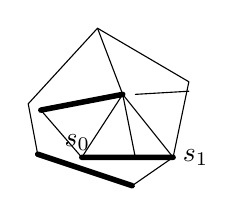
\begin{tikzpicture}[scale=.8,line cap=round,line join=round]
\draw (0,1.3)--(1.1,2.5)--(2.55,1.65)--(2.3,.45)--(1.65,0)--(.15,.5)--cycle;
\draw (1.1,2.5)--(1.5,1.45)--(.2,1.2)--(.85,.45)--(2.3,.45)--(1.5,1.45)--(.85,.45);
\draw (1.5,1.45)--(1.7,.45);
\draw (1.7,1.45)--(2.55,1.5);
\draw[line width=2pt] (.2,1.2)--(1.5,1.45) (.15,.5)--(1.65,0) (.85,.45)--(2.3,.45);
\node at (.78,.68) {$s_0$};\node[right] at (2.3,.45) {$s_1$};
\end{tikzpicture}}
\[
\begin{aligned}
s_0,\quad s_1&=\sigma_0s_0\\
s_2&=\sigma_1s_1\\
s_3&=\sigma_2s_2
\end{aligned}
\qquad
\begin{aligned}
f_1&=\mathrm{Dr}(s_0,s_1)\\
f_2&=\mathrm{Pl}(s_0,s_1,s_2)
\end{aligned}
\]
% middle left drawing
\figure{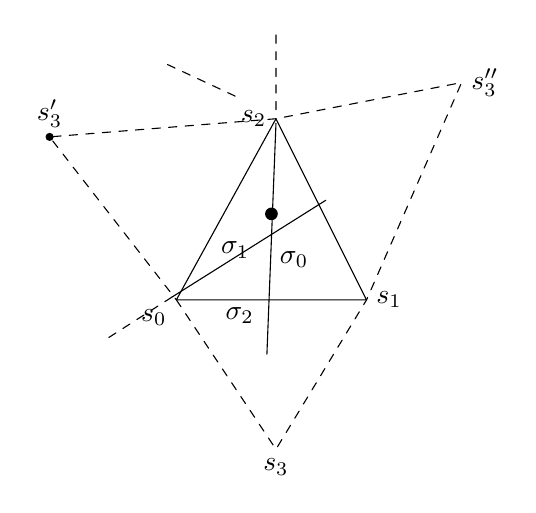
\begin{tikzpicture}[scale=1.15,line cap=round,line join=round]
\coordinate (a) at (0,0);\coordinate (b) at (2.1,0);\coordinate (c) at (1.1,2);
\draw (a)--(b)--(c)--cycle;
\draw[dashed] (a)--(1.1,-1.65)--(b)--(3.15,2.4)--(c)--(-1.4,1.8)--(a);
\draw[dashed] (1.1,2.1)--(1.1,3) (.65,2.25)--(-.1,2.6);
\draw (1,-.6)--(1.1,1.95) (-.05,.03)--(1.65,1.1);
\draw[dashed] (-.05,.03)--(-.8,-.45);
\fill (1.05,.95) circle(.07);\fill (-1.4,1.8) circle(.045);
\node[below left] at (a) {$s_0$};\node[right] at (b) {$s_1$};\node[left] at (c) {$s_2$};
\node[below] at (1.1,-1.65) {$s_3$};\node[above] at (-1.4,1.8) {$s'_3$};\node[right] at (3.15,2.4) {$s''_3$};
\node at (.65,.55) {$\sigma_1$};\node at (1.3,.45) {$\sigma_0$};\node at (.7,-.17) {$\sigma_2$};
\end{tikzpicture}}
\[
\left\{\begin{aligned}e_1&=s_1-s_0\\e_2&=s_2-s_0\\e_3&=s_3-s_0\end{aligned}\right.
\qquad
\begin{aligned}
\sigma_0:\quad&s_0\mapsto s_1\\&s_1\mapsto s_0\\&s_2\mapsto s_2\\&s_3\mapsto s_3\\[3pt]
\sigma_1:\quad&s_0\mapsto s_0\\&s_1\mapsto s_2\\&s_2\mapsto s_1\\&s_3\mapsto s'_3\overset{?}{=}\deleted{\unsure{s_3-|2s_3-}}\\[3pt]
\sigma_2:\quad&s_0\mapsto s_0\\&s_1\mapsto s_1\\&s_2\mapsto s_3\\&s_3\mapsto s_2
\end{aligned}
\]
\[
s'_3=s_0+\lambda e_1+\mu e_2+\nu e_3
\quad(=s_0+\lambda e_1-\unsure{\nu\lambda|\gamma\lambda}e_2+\nu e_3)
\]
% lower half
\[
\sigma_0:\left\{\begin{aligned}e_1&\mapsto-e_1\\e_2&\mapsto-e_1+e_2\\e_3&\mapsto\underline{-e_1+e_3}\end{aligned}\right.
\qquad
\deleted{\unsure{\text{et :}}}\quad
\sigma_0=\begin{pmatrix}-1&-1&-1&\unsure{1|0}\\0&1&0&0\\0&0&1&0\\0&0&0&1\end{pmatrix}
\]
\[
\sigma_1:\left\{\begin{aligned}e_1&\mapsto\deleted{\unsure{e_0|e_2}}\ e_2\\e_2&\mapsto e_1\\e_3&\mapsto\lambda e_1+\mu e_2+\nu e_3\\&\quad(=\lambda e_1-\lambda e_2+e_3\end{aligned}\right.
\qquad
\deleted{\unsure{\text{d'où}}}\quad
\sigma_1=\begin{pmatrix}0&1&\lambda&0\\1&0&\mu&0\\0&0&\nu&0\\0&0&0&1\end{pmatrix}
\]
\[
\sigma_2:\left\{\begin{aligned}e_1&\mapsto e_1\\e_2&\mapsto e_3\\e_3&\mapsto e_2\end{aligned}\right.
\qquad
\sigma_2=\begin{pmatrix}1&0&0&0\\0&0&1&0\\0&1&0&0\\0&0&0&1\end{pmatrix}.
\]
\scanpage{84}
% archive sheet number: 83
Écrivons \unsure{la relation|les relations}.
\[
\sigma_1^2=\mathrm{id}\qquad\unsure{\leftarrow}
\]
(les relations $\sigma_0^2=\sigma_2^2=\mathrm{id}$ et $\sigma_0\sigma_2=\sigma_2\sigma_0$ étant évidentes). Il suffit d'écrire
\[
\sigma_1^2(s_3)=s_3^{\unsure{*|4|' }}\qquad\text{i.e.}\qquad\sigma_1(s'_3)=s_3\qquad\text{or}
\]
\[
\begin{aligned}
\sigma_1(s'_3)&=\sigma_1s_0+\deleted{\unsure{\sigma_1e_3=s_0+\lambda}}\inserted{\lambda\sigma_1e_1+\mu\sigma_1e_2+\nu\sigma_1e_3}\\
&=s_0+\lambda e_2+\mu e_1+\nu(\lambda e_1+\mu e_2+\nu e_3)\\
&=s_0+(\mu+\nu\lambda)e_1+(\lambda+\nu\mu)e_2+\nu^2e_3
\end{aligned}
\]
\margin{$\lambda\ \mu\ \nu$}

Les conditions sont
\[
\left\{\begin{aligned}
\boxed{\begin{aligned}\nu^2&=1\\\mu&=-\nu\lambda\end{aligned}}
&\quad\begin{aligned}\deleted{\unsure{\mu+\nu\lambda=0}}\quad &(1^\circ)\\ &(2^\circ)\end{aligned}\\
\lambda=-\nu\mu\quad&\text{ou encore}\quad
\overset{\text{(compte tenu de }2^\circ\text{)}}{\lambda=\nu^2\lambda}\quad\text{qui résulte de }1^\circ,
\end{aligned}\right.
\]

Sur un corps, ces conditions se décomposent en deux possibilités
\[
\left\{\begin{aligned}\nu&=1,\ \mu=-\lambda\\\nu&=-1,\ \mu=\lambda\end{aligned}\right.
\]
% slanted
\margin{On peut \unsure{prouver} en tous les cas $\nu=1$, en écrivant $\unsure{u^3}=\mathrm{id}$ on aura $\unsure{u}s''_3=s'_3$ (où $s''_3=\sigma_0(s'_3)$) $\unsure{\ne|=}$ $\sigma_0\sigma_1s_3$ ou $\sigma_1s''_3=s'_3$, i.e. $\sigma_1\sigma_0\sigma_1(s_3)=\sigma_0\sigma_1(\unsure{s'_3|s_3})$ \unsure{---}}

Notons que
\[
\det\sigma_1=\deleted{\unsure{\det}}-\nu
\]
donc si on veut $\det\sigma_1=-1$ (\unsure{i.e.|c.à.d.|Ceci.} si on veut $\sigma_1$ une réflexion) on doit avoir $\nu=1$, $\mu=-\lambda$.

On aura alors \deleted{donc}
\[
s'_3-s_3=\deleted{\unsure{\lambda e_1+\mu e_2}}\inserted{\underbrace{(s'_3-s_0)}_{\unsure{u(e_3)}}\unsure{+|-}\underbrace{(s_3-s_0)}_{e_3}}=\lambda(e_2-e_1)=-\lambda(s_2-s_1)
\]
On \unsure{posera|pose}
\[
-\lambda=(1+\alpha)\qquad\lambda=-(1+\alpha)=\alpha'\tag*{(1)}
\]
de sorte qu'on aura
\[
s'_3-s_3=(1+\alpha)(s_2-s_1)\tag*{(2)}
\]
\scanpage{85}
% archive sheet number: 84
\unsure{Et} la matrice de $\sigma_1$ est.
\[
\sigma_1=\begin{pmatrix}0&1&-(1+\alpha)&0\\1&0&1+\alpha&0\\0&0&1&0\\0&0&0&1\end{pmatrix}
=\begin{pmatrix}0&1&\alpha'&0\\1&0&-\alpha'&0\\0&0&1&0\\0&0&0&1\end{pmatrix}\tag*{(3)}
\]
Posons
\[
\left\{\begin{aligned}
u_{\deleted{\unsure{0|1}}}&=\sigma_0\sigma_1
& s_0\mapsto s_1\mapsto s_2\mapsto\unsure{s_1|s_0},\ s_3\mapsto s''_3\deleted{\unsure{4}}\\
v_{\deleted{\unsure{1|2}}}&=\sigma_1\sigma_2
& s_0\mapsto s_0,\ s_3\mapsto s_1\mapsto s_2\mapsto s'_3
\end{aligned}\right.\tag*{(4)}
\]
\margin{à calculer $\unsure{\nwarrow}$}
\deleted{Notons que $\unsure{s_0},s_1,s_2,s_3$}

On aura
\[
\begin{aligned}
s''_3&=us_0+ue_3=s_{\unsure{1|2}}+\sigma_0(\sigma_1(e_3))=s_0+e_1+\sigma_0\bigl[(1+\alpha)(e_2-e_1)\\
&\hspace{10cm}+e_3\bigr]\\
&=s_0+e_1+(1+\alpha)\deleted{\unsure{(}}e_2\deleted{\unsure{-e_1)}}+e_3-e_1
\end{aligned}
\]
donc
\[
s''_3=s_0+(1+\alpha)\deleted{\unsure{(}}e_2\deleted{\unsure{-e_1)}}+e_3=s_3+(1+\alpha)e_2\tag*{(5)}
\]
Ou encore
\[
s''_3-s_3=(1+\alpha)(s_2-s_0)\tag*{(6)}
\]
\unsure{Notons|Calculons} $u(s'_3)$ utilisant (2)
\[
\deleted{us'_3=us_0+ue_3=s_1+\sigma_0\sigma_1\bigl((1+\alpha)(e_2-e_1)+e_3\bigr)=s_1+(1+\alpha)u(s_2-s_1}
\]
\[
\begin{aligned}
u(s'_3)&=u(s_3)+(1+\alpha)\underbrace{u(s_2-s_1)}_{s_0-s_2=-e_2}=s''_3-(1+\alpha)e_2\\
&\underset{\unsure{(5)|(6)}}{=}s_3
\end{aligned}
\]
\deleted{\unsure{au}} Enfin, on trouve de $\unsure{=|\text{même}}$ par (6),
\[
\deleted{\unsure{(7)}}\qquad\deleted{\unsure{u(s_3)\quad s_3\longrightarrow s'}}
\]
\[
\begin{aligned}
\deleted{\unsure{(7)}}\quad u(s''_3)&=u(s_3)+(1+\alpha)\overbrace{u(s_2-s_0)}^{s_0-s_1=-e_1}=s''_3-(1+\alpha)e_1\\
&=s_0+(1+\alpha)(e_2-e_1)+e_3
\end{aligned}
\]
\scanpage{86}
% archive sheet number: 85
donc
\[
u:\quad s_3\mapsto s''_3\mapsto s'_3\mapsto s_3\tag*{(7)}
\]
Donc on trouve
\[
u^3=\mathrm{id}\qquad\deleted{\unsure{u^2=1}}\quad(u\ne\mathrm{id}\ \text{bien sûr})\tag*{(8)}
\]
Notons que $s_3,s_1,s_2,s'_3$ sont dans un $=$ plan (celui d'équation $x+y+z=1$ !) et ce plan est stable par $\sigma_1$ et $\sigma_2$ (\unsure{idem|donc} par $v=\sigma_1\sigma_2$), \deleted{\unsure{aussi}} donc par \deleted{$\unsure{u}$}\inserted{$v=\sigma_1\sigma_2$}. Un calcul \unsure{connu|comme} montre que
\[
v^5=\mathrm{id}\quad\Longleftrightarrow\quad\boxed{\alpha^2+\alpha-1=0}\tag*{(9)}
\]
Donc si $G$ est le groupe
\[
\begin{aligned}
G&=\left\{\sigma_0,\sigma_1,\sigma_2\ \middle|\ \begin{aligned}&\sigma_0^2=\sigma_1^2=\sigma_2^2=1,\quad\sigma_0\sigma_2=\sigma_2\sigma_1,\\&(\sigma_0\sigma_1)^3=1,\ (\sigma_1\sigma_2)^5=1\end{aligned}\right\}\\
&=\mathrm{Aut}(\text{icosaèdre comb. épinglé}\ldots)
\end{aligned}\tag*{(10)}
\]
alors sous réserve que $\alpha^2+\alpha-1=0$, ce groupe \inserted{fini} $G$ opère \inserted{affinement} sur $\mathbb{E}^3$. Montrons que l'ensemble des transformés de $s_0$, $\mathrm{Dr}(s_0,s_1)$ et $\mathrm{Pl}(s_0,s_1,s_3)$ forme un icosaèdre géométrique ? Cela signifie que sur \unsure{tt|le} corps, les seules relations d'incidence entre ces \deleted{droites} sommets, droites et plans sont celles
\scanpage{87}
% archive sheet number: 86
de l'\unsure{icosaèdre}
\scanpage{88}
% archive sheet number: 87
de l'icosaèdre combinatoire.

Si nous admettons que $G$ est \inserted{fini} d'ordre $120$, comme le stabilisateur de $s_0$ contient le groupe \inserted{$\unsure{Z|\mathbb{Z}}$} engendré par $v$ (cyclique d'ordre $5$) en plus de $\sigma_1$ -- donc le groupe \unsure{diédral} $\{1,\sigma_1\}.Z$ (produit $1/2$ direct), on voit que le nb des sommets est un diviseur de $120/10=12$. Notons que les six points déjà écrits $s_0,s_1,s_2,s_3,\unsure{s'_3|s_3^*},s''_3$ sont \uline{distincts}, car leurs coordonnées sont
\diagram{\((11)\quad\left\{\begin{gathered}\begin{tikzcd}[ampersand replacement=\&,row sep=small,column sep=small]
s_0=(0,0,0)\arrow[d,bend left=60,leftrightarrow]\\
s_1=(\unsure{1|0},0,0)\\
s_2=(0,1,0)\arrow[d,bend left=60,leftrightarrow]\\
s_3=(0,0,1)\\
s'_3=(-(1+\alpha),1+\alpha,1)=(\deleted{\unsure{+}}\alpha',-\alpha',1)\\
s''_{\unsure{2|3}}=(0,1+\alpha,1)=(0,-\alpha',1)
\end{tikzcd}\end{gathered}\right.\)}
\margin{$\alpha'=-(\alpha+1)=-\alpha^{-1}$ (``l'autre racine'' de $\alpha^2+\alpha-1=0$)}

\deleted{\unsure{Il}} Il est clair que $s_0$ à $s_3$ sont tous distincts, il faut \deleted{voir} les comparer à $s'_3,s''_3$ et \unsure{comparer} entre eux. Comme la dernière coordonnée de $s'_3,s''_3$ \deleted{sont} est $1$, ils sont $\ne s_0,s_1,s_2$ dont la dernière coordonnée est nulle. Ils \deleted{ne peuvent être}\inserted{sont} égaux \inserted{l'un ou l'autre à} $s_3$ \deleted{\unsure{que ssi|que si}} $1+\alpha=0$\inserted{(i.e. $\alpha=-1$)}, qui est \inserted{donc} aussi la condition néc et suff. pour que $s'_3=s''_3$. Or \deleted{\unsure{$1+\alpha=0$}} si $\alpha=-1$
\scanpage{89}
% archive sheet number: 88
l'équation $\alpha^2+\alpha-1=0$ devient $-1=0$, qui n'est jamais vérifiée (sur une base non vide !). Cela \deleted{signifie}\inserted{implique} que le nb \unsure{de|des} \deleted{\unsure{pts est}}\inserted{sommets est} au moins six, donc égal à six ou douze. Si c'était \deleted{douze} six, le stabilisateur de \deleted{\unsure{$E$}}$s_0$ serait un groupe d'ordre $20$ contenant le groupe diédral \inserted{$D_5$} -- or il n'y en a qu'un seul, qui est le produit de $D_5$ par le centre $\unsure{\mathfrak{z}|z}=\{1,\underline{a}\}$\inserted{antipodisme}. On voit que cela signifierait que $as_0=s_0$, ou $as_3=s_3$ (cela revient au $=$ par homogénéité).

Nous allons donc calculer les antipodiques des $6$ points déjà marqués (\unsure{pour faire rapide}) -- ce qui nous donnera une liste des $12$ pts !

On va d'abord déterminer le \uline{centre} de l'icosaèdre, défini (s'il existe) comme l'unique (?) pt fixe \unsure{ss|sous} $G$.
\scanpage{90}
% archive sheet number: 89
% The writing occupies only the lower-right part of the sheet.
\[
\alpha+\alpha'=-1\qquad
\left\{\begin{aligned}\alpha&=-(\unsure{\alpha'}+1)\\\alpha'&=-(\alpha+1)\end{aligned}\right.
\]
\[
\alpha\alpha'=-1\qquad
\left\{\begin{aligned}\alpha&=-1/\alpha'\\\alpha'&=-1/\alpha\end{aligned}\right.
\]
\[
(1-\alpha)(1-\alpha')=1
\]
\[
(1+\alpha)\alpha=(1+\alpha')\alpha'=1\qquad(1+\unsure{\alpha|2})(1+\alpha')=-1
\]
\[
(\alpha+2)(\alpha'+2)=1
\]
\[
(2\alpha-1)(2\alpha'-1)=-1.
\]
\scanpage{91}
% archive sheet number: 90
\[
\left\{\begin{aligned}
\sigma_0(x,y,z)&=(\unsure{1-(x+y+z)},y,z)\\
\text{pts fixes définis par}\quad&\deleted{\unsure{x=-\tfrac12(y+z-1)}}\inserted{2x+y+z-1=0}\quad\text{(si }2\text{ inv)}
\end{aligned}\right.\tag*{(12)}
\]
\margin{\deleted{\uline{NB} en car. $2$, c'est l'hyperplan à l'infini}}
\[
\left\{\begin{aligned}
\sigma_1(x,y,z)&=(y-(1+\alpha)z,x+(1+\alpha)z,z)=(y+\alpha'z,x-\alpha'z,z)\\
\text{pts fixes définis par}\quad&\left\{\begin{aligned}
\underline{x+(1+\alpha)z=y}&\qquad\text{(\unsure{id.} en }x,y,z\text{)}\\
\deleted{\unsure{x-\alpha'z=y}}&\\
x-y-\alpha'z&=0
\end{aligned}\right.
\end{aligned}\right.\tag*{(13)}
\]
\[
\left\{\begin{aligned}\sigma_2(x,y,z)&=(x,z,y)\\\text{pts fixes définis par}\quad&y=z\end{aligned}\right.\tag*{(14)}
\]
\margin{$x=\frac12\alpha',\ y=\alpha'x=\deleted{\unsure{\frac{\alpha'^2}{2}}}\inserted{\frac{\unsure{1-\alpha'|-1-\alpha'}}2},\ z=y\unsure{\ne|=}\frac12$; \deleted{$\unsure{x=\frac\alpha2,\ y=z=-\frac1{2\alpha}}$}}

\uline{Centre} $o$ de coordonnées
\[
\deleted{\unsure{\tfrac12(\tfrac12\alpha',1,1)|\tfrac12(\alpha',1,1)}}
\]
\[
\deleted{\unsure{o=(\tfrac12,-\tfrac1{2\alpha},-\tfrac1{2\alpha})=\tfrac12(-1,-\tfrac1\alpha,-\tfrac1\alpha)}}
\]
\[
o=\frac12(\alpha',1-\alpha',1-\alpha')=\frac12(-(1+\alpha),2+\alpha,2+\alpha)\tag*{(15)}
\]

\uline{NB} l'équation $\alpha^2+\alpha-1$ implique $\alpha$ inv. et \deleted{en fait $\unsure{\Rightarrow|=}$} elle s'écrit
\[
\boxed{\alpha(\alpha+1)=1}\qquad\unsure{\text{or}|\text{ou}}\tag*{(16)}
\]
\deleted{On a $\alpha-2$ \unsure{pas inv.}}

[en fait, $\alpha(\alpha+1)(\alpha-1)(\alpha+2)\inserted{(2\alpha-1)}$ \unsure{sera} inv. $\unsure{\ldots\}}$, et $(\alpha-2)$ sera inv. ssi $5$ est inv.\dots]

Ainsi, en car. $\ne2$ le centre est donné par les coordonnées (15), et en car. $2$ c'est \inserted{sans doute} le pt à l'infini dans la direction $(-1,\frac1\alpha,\frac1\alpha)$\dots\ ].
\scanpage{92}
% archive sheet number: 91
Ceci dit, on doit pouvoir \inserted{sans mal} vérifier ceci

\uline{Prop} l'antipodisme $\underline{a}$ est la symétrie \unsure{par r. au|par au} pt $o$ donné par (15)\inserted{si $2$ inv.}, et dans tous les cas il est donné par la formule
\[
\underline{a}(x,y,z)=(\alpha'-x,(1-\alpha')-y,(1-\alpha')-z)\tag*{(17)}
\]
\[
\deleted{\unsure{=(\alpha'-x,-(1+\alpha)-y,\alpha+2-z)}}
\]
Si $2$ est inv., \deleted{$\unsure{a}$}\inserted{$\underline{a}$} a $o$ comme unique pt fixe -- or les $s_i,\deleted{\unsure{s_3}},s'_3,s''_3$ sont $\ne o$ (n'étant pas fixes sous $G$) En car. \deleted{\unsure{zéro}} $2$, $\underline{a}$ est la translation par le vecteur $(\alpha',1,1)$, donc n'a pas de pt fixe (à distance finie).

\uline{NB} En car. $2$, \unsure{\deleted{les solutions}|\uline{les solutions}} de l'équation $\alpha^2+\alpha-1=0$ sur une ext. \inserted{alg. clos. $K$} de $\mathbb{F}_2$ sont les deux éléments de $\deleted{\unsure{\mathbb{F}_4}}\unsure{\mathbb{F}_4}.\ \unsure{\widetilde{K}\setminus K}$, où $\unsure{K|\widetilde{K}}$ est l'unique ext. quadratique de $\mathbb{F}_2$ dans $K$. \unsure{Si on pose}
\[
\mathbb{F}_4\overset{\unsure{\text{déf}|\text{dfn}}}{=}\mathbb{F}_2[T]/(T^2+T+1)=\begin{gathered}\text{corps des racines}\\\text{primitives }3^{\text{èmes}}\text{ de}\\\text{l'unité sur }\unsure{\mathbb{F}_2|\mathbb{F}_p}\end{gathered}
\]
la donnée d'un $\alpha$ sur $S/\mathbb{F}_2$ \unsure{satisfaisant} l'équation $\alpha^2+\alpha-1=0$ équivaut à la donnée d'une $\mathbb{F}_4$-structure sur $S$, i.e. d'un morphisme $S\longrightarrow\operatorname{Spec}\mathbb{F}_4$. Notons que $\alpha^2=\frac1\alpha=\alpha+1$ est l'\uline{autre} él. de $\mathbb{F}_4\setminus\mathbb{F}_2$.
\scanpage{93}
% printed form: music staves without printed text.
\[
\left\{\begin{aligned}
\underline a s_0&=(\alpha',1-\alpha',1-\alpha')\\
\underline a s_1&=(\alpha'-1,1-\alpha',1-\alpha')\\
\underline a s_2&=(\alpha',-\alpha',1-\alpha').\\
\underline a s_3&=(\alpha',1-\alpha',-\alpha')\\
\underline a s_3'&=(0,1\deleted{\unsure{-\alpha'}},-\alpha').\\
&\deleted{\unsure{1-2\alpha+3|2\alpha+3}}\\
\underline a s_3''&=(\alpha',1\deleted{\unsure{-\alpha'}},-\alpha').
\end{aligned}\right.
\tag*{(18)}
\]
% archive sheet number: 92
\scanpage{94}
\deleted{Écrivons les antipodiques des $s_i,s_3',s_3''$}
\[
\left\{\begin{aligned}
&\deleted{\underline a s_0=(1,-\frac1\alpha,-\frac1\alpha)=(1,-1-\alpha,-1-\alpha)=(1,\unsure{\alpha'},\alpha')}\\
&\deleted{\underline a s_1=(0,-\frac1\alpha,-\frac1\alpha)=(0,-1-\alpha,-1-\alpha)=(0,\alpha',\alpha')}\\
&\deleted{\underline a s_2=(1,-\frac1\alpha-1,-\frac1\alpha)=(1,-2-\alpha,-1-\alpha)=(\unsure{1|\alpha'},\alpha'-1,\alpha')}\\
&\deleted{\underline a s_3=(1,-\frac1\alpha,-\frac1\alpha-1)=(1,-1-\alpha,-2-\alpha)=(1,\alpha',\alpha'-1)}\\
&\deleted{\underline a s_3'=(2+\alpha,-2(1+\alpha),-(2+\alpha))=(1-\alpha',-2\alpha',\alpha'-1)}\\
&\deleted{\underline a s_3''=(1,-2(1+\alpha),-(2+\alpha))=(1,2\alpha',\alpha'-1)}
\end{aligned}\right.
\tag*{\deleted{(18)}}
\]
% Horizontal separator below the cancelled calculation, arrow at its left end.
\figure{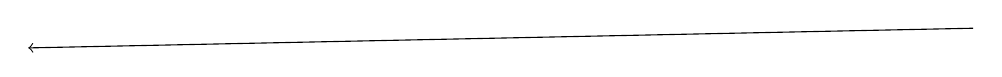
\begin{tikzpicture}\draw[<-] (0,0)--(12,.25);\end{tikzpicture}}

On aimerait prouver que \inserted{(sur un corps de base \unsure{quelc.})} trois \deleted{pts} \inserted{sommets} distincts \inserted{(\unsure{ce qui implique|non antipodiques} \unsure{provenant d'une arête|incidents à une arête} \unsure{par un pt donné})} ne sont pas alignés, et quatre points distincts ne sont pas \deleted{sur} \inserted{ds} un $=$ plan \uline{sauf} s'ils \deleted{appartiennent à une face} sont incidents \inserted{combinatoirement} à un $=$ sommet (ce qui implique qu'un sommet n'est incident \inserted{géom\textsuperscript{t}} à une face que s'il \deleted{elle} l'est combinatoirement; et \inserted{par suite} qu'une arête n'est incidente \inserted{géom\textsuperscript{t}} à une face que si elle est incidente combinatoirement).
\margin{?}
\margin{C'est en tous cas \uline{faux} en car. 2 !}
\figure{\begin{tikzpicture}\fill (0,.5) circle (1.5pt);\draw[->] (.15,.5)--(1.4,.55);\fill (0,0) circle (1.5pt);\draw (0.15,0)--(1.4,.1);\draw[->] (.7,1.4)--(2,2.6);\draw (1.95,2.75)--(1.75,5.2);\end{tikzpicture}}

Pour le premier pas, il y a trois vérifications à faire

\unsure{a)} La droite qui joint $s_0$ à son antipodique $\underline a s_0$ ne contient aucun autre sommet. i.e. \unsure{aucun des|aucun que les} \inserted{10} vecteurs \deleted{\unsure{tq}} \inserted{$(x,y,z)$} associés aux dix sommets distincts de $\unsure{s_3|s_0},\underline a s_0$, sont non prop. \unsure{au Centre|au vecteur}
\[
\underline a s_0=(\alpha',1-\alpha',1-\alpha')\deleted{\unsure{=(1,-1-\alpha,-1-\alpha)}}
\]
ou encore à
\[
\frac1{\unsure{\alpha'}}\underline a s_0=(1,\alpha',\alpha')
\]
% archive sheet number: 93
\scanpage{95}
\uline{\unsure{OK|Or}} C'est vrai.
\margin{$\unsure{*}$}

b) La droite joignant $s_0$ à $s_1$ ne contient pas d'autre sommet, i.e. les 10 \deleted{vecteurs}-sommets distincts de $s_0,s_1$ sont non prop. à $s_1=(1,0,0)$.

C'est vrai.

c) La droite joignant $s_0$ à $s_3''$ ne contient pas d'autre sommet, i.e. les 10 \unsure{aut. som.} distincts de $s_0,s_3''$ sont non prop. à
\[
s_3''=(0,1+\alpha,1)
=(0,-\alpha',1)
\]
C'est vrai.

Le deuxième pt semble plus fastidieux. Mais si on est \unsure{seulement} intéressé au cas de 4 pts \inserted{distincts} dont trois forment face, on est ramené à ceci :

Aucun des 9 autres sommets distincts de $s_0,s_1,s_2$ n'est dans le plan qu'ils engendrent, i.e. n'a de coordonnée $z$ nulle. Or c'est vrai -- et on est heureux !
% archive sheet number: 94
\scanpage{96}
Fonctions \unsure{quadr.} invariantes
\[
f(x,y,z)=ax^2+by^2+cz^2+u\unsure{yz}+\unsure{v|\nu}\unsure{zx}+wxy+\lambda x+\mu y+\nu z+d
\]
Comme les c\textsuperscript{tes} sont invariantes, \unsure{SPS} $d=0$

L'invariance par $\sigma_2:(x,y,z)\unsure{\vdash|\longmapsto}(x,z,y)$ signifie $b=c$, $v=w$, $\mu=\nu$ i.e.
\[
f(x,y,z)=ax^2+\deleted{b\underbrace{(y^2+z^2)}}+\deleted{u\underbrace{yz}}+vx(y+z)+\lambda x+\deleted{\mu\underbrace{(y+z)}}
\]
Faisons la substitution $\sigma_0:(x,y,z)\vdash(1-(x+y+z),y,z)$
\[
\begin{aligned}
f\circ\sigma_0(x,y,z)
&=a(\underset{\unsure{\times|\checkmark}}1+\underset{\times}{x^2}+\underset{\times}{y^2}+\underset{\times}{z^2}+\underset{\times}{2yz}+\underset{\times}{2zx}+\underset{\times}{2xy}-2(\overset{\times}x+\overset{\times}y+\overset{\times}z))\\
&\quad+\deleted{b(y^2+z^2)}+\deleted{uyz}+v(1-\overbrace{(x+\underbrace{y+\underbrace{z))(y}+z}})\\
&\quad+\lambda(1-(\underset{\times}x+\underset{\times}y+\underset{\times}z))+\deleted{\mu(y+z)}\\
&=ax^2+(\deleted b+a\inserted{\unsure{+v|-v}})(y^2+z^2)+(\deleted u+2a\deleted{\unsure{y|v}}-2v)yz\\
&\quad+\unsure{(}2a-v)x(y+z)+(-2a-\lambda)x\unsure{\circ|0}\\
&\qquad+(-2a-\lambda+\deleted\mu\inserted{+v})(y+z)+(a+\deleted{\unsure{u|v}}+\lambda)
\end{aligned}
\]
d'où
\[
\begin{aligned}
&\boxed{\unsure{v}=a}\\
&2v=2a\quad\text{ok}\\
&2a-v=v\quad\text{ok}\\
&-2a-\lambda=\lambda\quad\text{i.e.}\quad\lfloor\underline{2}(\lambda+a)=0\\
&\mu=-2a-\lambda\inserted{+v}+\mu\quad\text{i.e.}\quad\boxed{\lambda=-a}\quad\underset{\text{(comme }v=a\text{)}}{}
\end{aligned}
\]
\diagram{\begin{tikzcd}[ampersand replacement=\&,column sep=large]
{}\arrow[r,bend right=15]\&\deleted{\unsure{2\lambda+2a=0}}\quad\boxed{\deleted{\unsure{2\lambda+2a=0|\lambda+2a=0}}}
\end{tikzcd}}
\[
\deleted{a+\underset{\substack{\parallel\\a}}v\unsure{+|=}\lambda=0\quad\lambda=\unsure{2a|-2a}\quad\text{ok}}
\]
\[
f(x,y,z)=ax^2+b(y^2+z^2)+uyz+ax(y+z)\inserted{-ax}+\mu(y+z)
\]
\margin{$\boxed{\unsure{2a=0}}$}
\[
\begin{aligned}
&\deleted{=ax(x+y+z)+b(y^2+z^2)+uyz+\mu(y+z)}\\
&\deleted{\unsure{=a[x^2+x(y+z)-x]}}
\end{aligned}
\]
\[
f(x,y,z)=ax(x+y+z-1)+b(y^2+z^2)+uyz+\mu(y+z)
\]
% archive sheet number: 95
